\documentclass[11pt]{article}

\usepackage{a4wide}
\usepackage{mathptm}
\usepackage{xspace}
\usepackage{amsmath}
\usepackage{graphicx}
\usepackage{algorithm}
\usepackage{algpseudocode}
\usepackage{tikz}
\usepackage{tkz-graph}
\usetikzlibrary{shapes.misc, positioning}
\usepackage{listings}
\usepackage{color}
\usepackage{hyperref}

\definecolor{dkgreen}{rgb}{0,0.6,0}
\definecolor{gray}{rgb}{0.5,0.5,0.5}
\definecolor{mauve}{rgb}{0.58,0,0.82}

\lstset{frame=tb,
  language=Java,
  aboveskip=3mm,
  belowskip=3mm,
  showstringspaces=false,
  columns=flexible,
  basicstyle={\small\ttfamily},
  numbers=left,
  numberstyle=\tiny\color{gray},
  keywordstyle=\color{blue},
  commentstyle=\color{dkgreen},
  stringstyle=\color{mauve},
  breaklines=true,
  breakatwhitespace=true,
  tabsize=3
}
\begin{document}

\title{DAT250 - FeedApp}

\author{Adrian Lind Bergersen, Nicolas Eduardo Motamayor Aguiton, Philip Lindstøl Svenningsen, and Jacob Haile Yebio}

\maketitle

\begin{abstract}

  10-15 lines with the software technology and the highlights from the
  project that has been undertaken.

\end{abstract}

%\input{commands}

\section{Introduction}
\label{sec:introduction}

The FeedApp project was developed as part of the DAT250 Advanced Software Technologies course to explore innovative solutions for managing polling systems effectively. The primary motivation was to create a scalable, secure, and user-friendly application for conducting polls while integrating advanced software technologies and best practices. This project addresses challenges such as ensuring reliable voting mechanisms, securing user data, and providing real-time analytics for decision-making.

The FeedApp allows users to create polls, vote, and view results through an intuitive web interface. Its design incorporates modern development practices such as RESTful APIs, microservices architecture, and CI/CD pipelines to ensure reliability and maintainability. By leveraging a relational database for core application data and a NoSQL database for analytics, the system is optimized to handle both structured and unstructured data efficiently. Furthermore, the inclusion of messaging systems for asynchronous communication enables real-time processing and storage of aggregated voting data.

A unique aspect of the FeedApp is its front-end implementation using the Elm programming language. Elm’s functional programming paradigm ensures a type-safe and error-free development environment, making it ideal for building high-reliability web applications. The project also integrates widely-used technologies like Java/SpringBoot, RabbitMQ, and MongoDB, chosen for their reliability, scalability, and compatibility.

The remainder of this report is structured as follows: First, we detail the FeedApp’s design and use cases, followed by an in-depth discussion of its architecture and technology stack. Next, we examine the prototype implementation and evaluate the project’s outcomes. Finally, we reflect on lessons learned and evaluate the effectiveness of the chosen technologies.

Through this report, we aim to present a comprehensive overview of the FeedApp, highlighting the challenges faced during its development and the solutions that emerged. The insights gained from this project demonstrate the potential of combining modern technologies to solve real-world problems in software development.



\usepackage{float}

\section{Design}
\label{sec:design}

\subsection{Use Cases}
The use cases of the Feed App are quite simple in nature and do not require a large amount of explanation. However, before we dig into the details of the use cases, it is important to note that certain functionalities are locked to whether you are a registered user or not.

\subsubsection{Create Poll}
This part lets registered users create polls consisting of:
\begin{itemize}
    \item \textbf{PollID}: An automatically generated identifier for the polls that is used for request-logic such as updating, getting, and deleting the poll later on.
    \item \textbf{Title/Question}: This is the question that the registered user wants to ask the voters.
    \item \textbf{Options}: These consist of all the options that the creator wants to give the voters to vote on.
\end{itemize}

\subsubsection{Vote on Poll}
When it comes to voting on polls, it is restricted to registered users only, and therefore anyone who wants to vote will have to create an account in the app. The polls that the users vote on will consist of a question, and then the voting options accompanied by the current amount of votes. 

There is, however, a discussion to be made around whether or not the current votes should be public before making a vote, as this can sway the user into voting something that they might not have otherwise. On the other hand, having the votes public from the start will make sure that everything is transparent for the voters and also keep them as informed as possible.

\subsubsection{See Poll}
For the visibility of the polls on the website, there was no real reason to gatekeep what the available polls on the site look like. Therefore, both registered and unregistered users can see and read the polls that have been created by the registered users.

\subsubsection{Create Account}
Creating an account is an action that is required to do in order to create and vote on polls on the app. The act of creating an account requires the unregistered user to put in their login details that will consist of a name, password, and email.

\subsubsection{Log into Account}
For the last use case, there is the functionality of logging into the created accounts. This simply requires the registered user to type in the details used to create their account, and they will then be fully logged in and ready to use all the functionalities that the app has to offer in the UI.

\begin{figure}[thb]
	\centering
	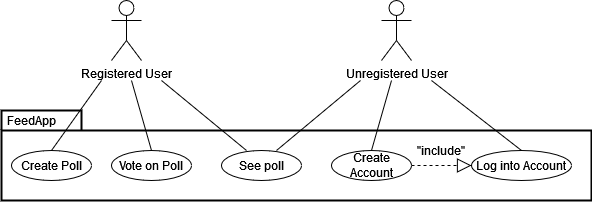
\includegraphics[scale=0.5]{figs/usecases.png}
	\caption{Use cases of the FeedApp.}
	\label{fig:usecases}
\end{figure}

\subsection{Domain Model}
This section will describe the domain model.

\subsection{Architecture}

\subsubsection{Web UI / Elm}
The web UI of the feed app is also the featured technology of this project. Therefore, it will be covered later on in a more in-depth look into the implementation and choice of the Elm programming language as our frontend framework for our web UI.

\subsubsection{REST API / Spring Web MVC}
The REST API works as the middleman between the frontend and backend as a way to perform all the CRUD operations in the application. This means that the integration of the REST API allows us to POST, UPDATE, GET, and DELETE data about the users and polls.

When it comes to the choice of using Spring Web MVC to implement this, there was not any good reason for us to change as the entire team has experience using it, and it also works seamlessly with the rest of the stack, as the Spring Web MVC is a dependency from the Spring Framework, which also has dependencies for Java, JPA, H2, RabbitMQ, and MongoDB. 

\subsubsection{Business Logic / Java}
For the business logic part of the project, we chose to go with Java for the simple reasons of reliability, familiarity, and possibilities. In other words, the entire group has experience working with Java, and the language gives us everything we need to create the feed app that we want. It also integrates well with the other components of the app, for example through the use of Spring Framework.

Alternatives would be to go the same route as mentioned in the section about alternatives for REST API, in other words the alternatives were other big enterprise languages such as Python, JavaScript, Ruby, and Kotlin. 

\subsubsection{Persistence \& Relational Database / JPA \& H2}
JPA (Java Persistence API) is the technology that connects our business logic with our relational database, which in this case is H2. JPA makes it possible to map Java objects to database tables, and it also allows us to do CRUD operations directly on our Java objects. 

The reason that the group went with JPA is that it also has a dependency and operability with Spring Framework, which makes it integrate easily and just work really well with the rest of our chosen stack.

When it comes to the choice of H2 for our database, it also works really easily and well because of its integration with the Spring Framework. In addition, it is a very simple and easy-to-learn database that gives us everything we need. One of the reasons we didn't need to go for any more complex databases, is that we also have an analytics component that gives us insight into the app’s data through its use of MongoDB as a non-relational database.

\subsubsection{Message Broker / RabbitMQ}
The message broker is one of the two parts that make up the analytics component of the project. The purpose of this message broker is to give us asynchronous communication between the feed app (business logic) and the database in the analytics component, which means that we don’t need real-time conversation to have interaction between the app and the analytics component. 

The positive side of doing this is that no messages will be lost, and that they are processed in the order they are sent by message queues in RabbitMQ. Message queues are simply a message that is stored for an indefinite time until it is processed, and then deleted from the queue.

The reason we chose RabbitMQ for message handling is that it supports the publish/subscribe model that we wanted to implement in our feed app, and it is also supported in Spring Framework through Spring AMQP, which makes it integrate very well with the rest of the stack.

Alternatives that we looked at were Apache Kafka and Redis, however they either provided too much unnecessary complexity (Kafka) or didn't offer the robustness that we needed (i.e Redis didn’t offer automatic re-delivery). Also the group had experience using RabbitMQ from earlier, so there was no real incentive to go for anything other than RabbitMQ, as it provided us all the functionality and ease-of-use that we needed for a message broker.

\subsubsection{Non-relational Database / MongoDB}
The non-relational database is the second part of the application’s analytics component, and is used to store all the data in an analytics-collection. This is then used to understand voting patterns, typical questions, and can be used to just learn more about the users of the feed app in general.

When it comes to the choice of MongoDB as the database, it was not a straightforward choice. We also had a serious look at Apache Cassandra and even possibly using Redis as the non-relational database. Both of these offered perks that we could not get with MongoDB, such as Apache Cassandra offering really good scalability and working very well with big data. Redis on the other hand can be used as a very lightweight and high-speed database that stores data in memory and also has built-in pub/sub functionality (meaning it can be used as both a message broker AND non-relational database), which makes it very easy and beginner-friendly to implement. Even though these two alternatives provide some good perks of use, there are still good reasons to pick MongoDB over them, and also it provides sort of a middle ground between Cassandra and Redis. The reason we decided to go for MongoDB was that it works for everything we need, which is to view our analytics in a simple document-model. It gives us a simplicity and ease-of-use that Cassandra cannot deliver, and also it lets us view our analytics in a way that Redis cannot deliver as easily (for example the use of complex queries like “find()” from MongoDB is not provided in Redis).

\begin{figure}[H]
	\centering
	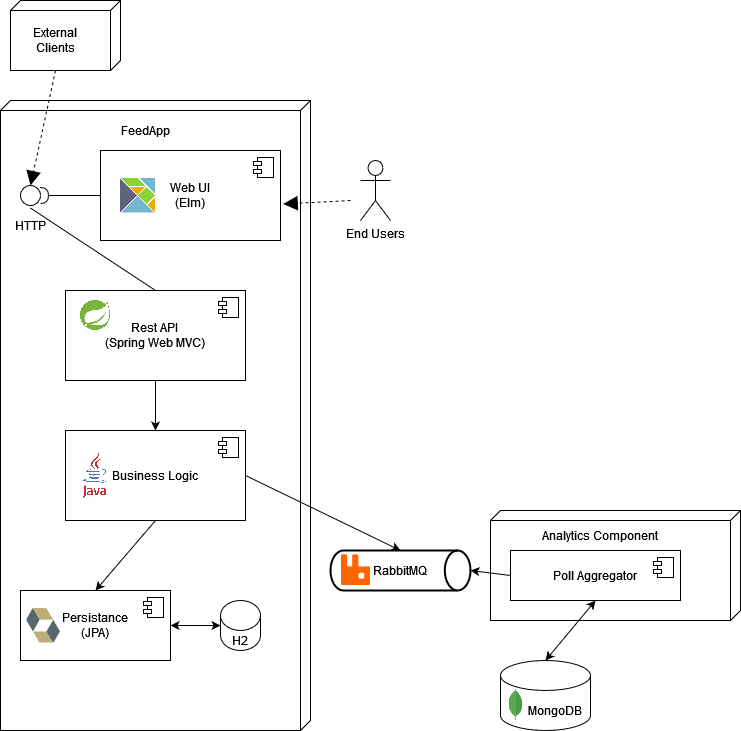
\includegraphics[scale=0.5]{figs/DAT250architecture.png}
	\caption{The software architecture of the FeedApp.}
	\label{fig:DAT250architecture}
\end{figure}


\section{Technology Assessment}
\label{sec:technology}

Elm was created by Evan Czaplicki in 2012 and was designed to simplify front-end development. By addressing common issues such as runtime errors and large, complex codebases, Czaplicki envisioned a tool that prioritised developer productivity and application reliability. This was achieved by combining the principles of functional programming with a focus on usability. Elm eliminates entire classes of runtime errors through its type-safe design while producing highly optimised and minimalistic deployment bundles. Its philosophy emphasises simplicity, predictability, and a delightful developer experience.

\begin{figure}[thb]
	\centering
	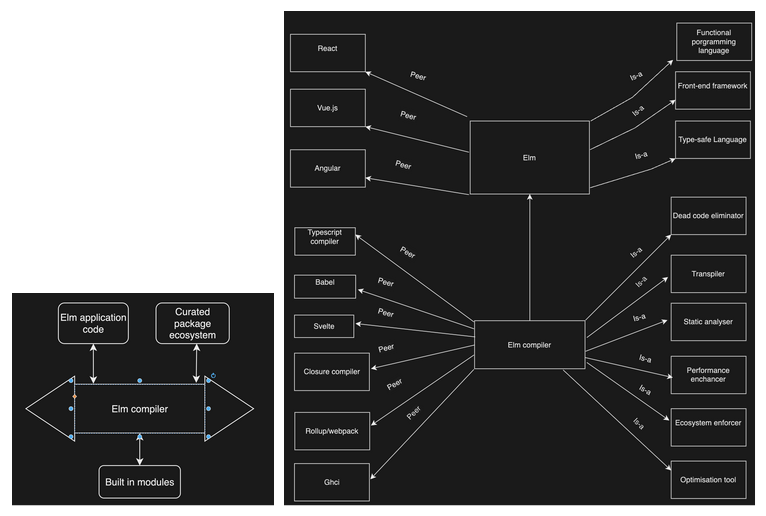
\includegraphics[scale=0.5]{figs/diagram.png}
	\caption{Figure.}
	\label{fig:diagram}
\end{figure}

\subsection{Elm's Ecosystem}
Figure 3 illustrates the key elements of Elm’s ecosystem. At its center is the \textbf{Elm Compiler}, which links application code, built-in modules, and a curated package ecosystem. This integration allows Elm to streamline and optimise the code it generates. Unlike frameworks like React or Angular, there is no dependence on separate build tools, as Elm’s compiler performs all optimisations directly, including removing unnecessary dependencies to reduce deployment size.

Figure 4 highlights Elm's relationships within the broader genealogy. Elm \textit{"is-a"} functional programming language and front-end framework. It emphasises immutability and type safety, setting it apart from traditional frameworks. Elm’s compiler also serves as a peer to tools like the TypeScript Compiler, Babel, and Svelte. While these tools aim to optimise and transform code, Elm’s compiler enforces consistency across its ecosystem, helping produce smaller and more predictable deployment bundles.

\section{Problem Domain Habitat}
Elm addresses significant challenges in front-end development. Managing application complexity, ensuring runtime reliability, and producing efficient deployment bundles are all areas Elm seeks to improve. Its approach is particularly suited to environments where application reliability and asset size are critical considerations. Unlike frameworks like React and Angular, which rely heavily on runtime libraries, Elm's architecture eliminates runtime exceptions through compile-time guarantees.

\begin{figure}[thb]
	\centering
	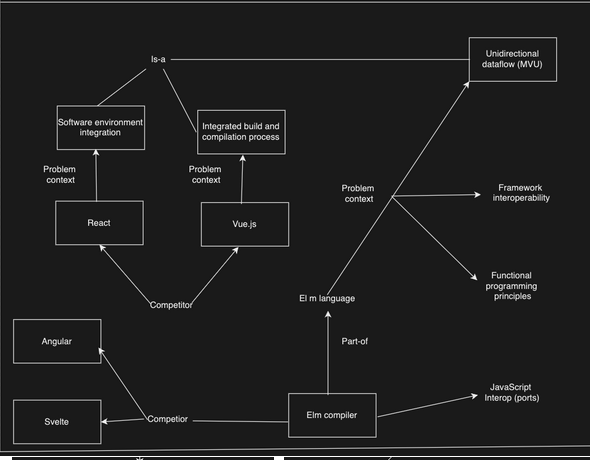
\includegraphics[scale=0.5]{figs/diagram2.png}
	\caption{Figure.}
	\label{fig:diagram2}
\end{figure}

Figure 5 depicts Elm competing with React, Vue.js, Svelte, and Angular in the domain of front-end frameworks. These tools address common issues such as state management, component reuse, and rendering efficiency. Elm distinguishes itself through its \textbf{Model-View-Update (MVU)} architecture, enforcing unidirectional data flow. This simplifies application logic and enables the compiler to produce highly optimised and minimalistic outputs.

Additionally, Elm supports JavaScript interoperability via \textbf{ports}, allowing integration with existing JavaScript codebases. This makes it feasible for developers to adopt Elm incrementally within larger applications. However, Elm’s curated package ecosystem and strict typing model put emphasis on stability over flexibility, distinguishing it from competitors that prioritise rapid prototyping or experimental features.

Elm excels in scenarios where predictable performance, maintainability, and minimal runtime overhead are critical, such as performance-critical web applications or bandwidth-constrained environments. Conversely, Elm’s limited ecosystem flexibility may be less suitable for projects needing extensive third-party library support.

\section{Experiment Design Phase}

\subsection{Comparative Feature Analysis}
The comparative feature analysis examines the features influencing deployment asset size in Elm, React, Vue, and Svelte. The reference model focuses on features that impact deployment size, including:

\begin{itemize}
    \item \textbf{Code Optimization:} Elm's compiler removes unused code and generates efficient JavaScript. React, Vue, and Svelte rely on external build tools like Webpack, which require proper configuration to avoid unused dependencies.
    \item \textbf{Dependency Management:} Elm uses a curated package system to reduce unnecessary libraries. React, Vue, and Svelte allow broader use of third-party dependencies, increasing the risk of bloated deployment assets.
    \item \textbf{Runtime Overhead:} Elm's functional programming model avoids runtime processes for dynamically updating the user interface, resulting in smaller runtime sizes. Svelte employs a similar compile-time approach. React and Vue use runtime processes to track and update changes, increasing final application size.
    \item \textbf{State Management:} Elm's MVU architecture simplifies state management at compile time, reducing runtime overhead. React uses unidirectional data flow with hooks and stateful components, Vue offers reactive data binding, and Svelte compiles reactive assignments into efficient JavaScript.
    \item \textbf{JavaScript Integration:} Elm uses \textit{ports} for JavaScript integration, which can slightly increase bundle size in hybrid apps. React, Vue, and Svelte natively integrate with JavaScript, but bundle size increases with multiple libraries.
\end{itemize}

\subsection{Feature Deltas}
Feature deltas highlight how Elm integrates its language, architecture, and compiler to reduce redundant dependencies and produce smaller bundles. React, Vue, and Svelte focus on runtime flexibility, often leading to larger deployment assets.

\subsection{Hypothesis Formulation}
From the analysis, the following hypothesis is formulated:
\begin{quote}
    \textit{"Applications written in Elm produce smaller deployment assets compared to applications written in popular frameworks like React, Vue, or Svelte for equivalent functionality."}
\end{quote}

The hypothesis is supported by:
\begin{enumerate}
    \item \textbf{Integrated Compiler:} Elm’s compiler optimises code at the source, reducing reliance on external tools.
    \item \textbf{Curated Ecosystem:} Elm's package system includes only essential libraries, avoiding unnecessary dependencies.
    \item \textbf{Functional Design:} Elm's declarative style and MVU model reduce redundant code and ensure smaller deployment assets.
    \item \textbf{Feature Deltas:} Elm prioritises efficiency compared to the runtime-heavy approaches of React, Vue, and Svelte.
\end{enumerate}

\subsection{Experiment Design}
The experiment involves two main approaches: \textbf{synthetic benchmarks} and a \textbf{demonstrator study}.
\begin{itemize}
    \item Synthetic benchmarks involve creating naive implementations of simple applications (e.g., "Hello World," counter, GET request) in Elm, React, Vue, and Svelte. These are used to compare how deployment assets scale with increasing complexity.
    \item The demonstrator study assesses Elm's functionality through the development of a poll application, evaluating lessons learned, compatibility with JavaScript applications, and the consequences of Elm’s unique features.
\end{itemize}

\section{Experiment Evaluation Phase}


\subsection{Synthetic Benchmarks}
The benchmarks revealed that Elm's asset size grows more rapidly compared to other frameworks. While Elm eliminates unused dependencies, its need to explicitly import common features (e.g., HTML elements, HTTP requests) increases the number of dependencies in each application, resulting in larger asset sizes. Conversely, React, Vue, and Svelte include these features in their core libraries, maintaining relatively constant sizes.

\begin{figure}[thb]
	\centering
	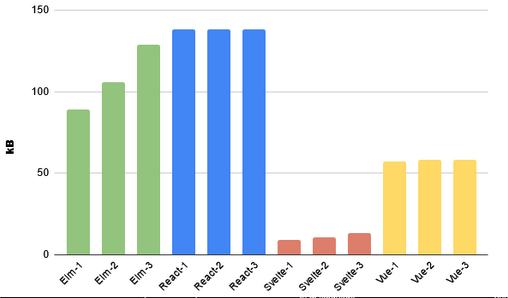
\includegraphics[scale=0.5]{figs/diagram3.png}
	\caption{Figure.}
	\label{fig:diagram3}
\end{figure}

\subsection{Demonstrator Study}
\textbf{General Observations:} Elm's steep learning curve posed challenges, especially for developers new to its architecture. While feature development was slower, its functional programming paradigm ensured reliability.

\textbf{Results:} Elm’s deployed site had an average page size of \textasciitilde 140kB. Consolidating pages into a single SPA could potentially save up to 60\% of the asset size by sharing common imports. The demonstrator study highlighted the importance of Elm's port and subscription system for interoperability with JavaScript applications, such as local storage access.

While the study discredits Elm's size advantage, it reinforces Elm’s strengths in reliability and maintainability through its type-safe, compiler-driven architecture.


\section{Prototype Implementation}
\label{sec:implementation}

This section should provide brief details of how the prototype has been implemented.
You may want to use come code snippets here, but only focus on core features and aspects.
You are not meant to copy/paste your whole application code into the report.
Focus for instance how other developers may run your application and how they might develop it further...


The example below shows how you may include code. There are similar
styles for many other langages - in case you do not use Java in your
project. You can wrap the listing into a figure in case you need to
refer to it. How to create a figure was shown in Section~\ref{sec:technology}.



\section{Conclusions}

Our goal with this project was to develop a simple poll application with an entire application stack. In addition it was our goal to evaluate our chosen featured technology, Elm. Though we did encounter some issues. Primarily that due to time constraints, we failed to stitch together the final application stack into a valid docker image. We did manage to implement all the discrete elements of our application. In addition we were able to evaluate our featured technology, though our hypothesis did not end up holding much water. Though this can teach us about the importance of actually evaluating our assumptions about a chosen technology, instead of simply relying upon the statistics we have available. 

References:

- Brown, A. W., & Wallnau, K. C. (1996). A framework for evaluating software technology (CMU/SEI-96-TR-010). Software Engineering Institute, Carnegie Mellon University.

\bibliographystyle{plain}
\bibliography{report.bib}{}

\end{document}
